\section{Introduction} % Include localisation techniques
\noindent
Cancer is one of the leading causes of death worldwide with around 20 million cases reported in 2022 - corresponding to around one in five men or women developing cancer in their lifetime \cite{bray_global_2024}. The conventional method for cancer diagnosis includes taking a biopsy of suspect tissue from a patient during surgery, and then subsequent pathological analysis. This pathological analysis generally involves staining of the biopsy with haematoxylin and eosin (HE). The haematoxylin stains nucleic acids a deep blue-purple colour, whilst the eosin is pink and non-specifically stains proteins \cite{fischer_hematoxylin_2008}. These HE stained samples can then be used by a pathologist to perform diagnosis. This process is manual, error-prone, subjective, costly, and time-consuming; often requiring transport to a laboratory for processing by highly trained technicians \cite{hollon_near_2020}. The time between pathologists receiving samples and a diagnosis being returned to a surgeon is often around 20 minutes \cite{novis_interinstitutional_1997} - any reduction in this processing time would therefore help to guide surgeries more effectively.\\

New methods are being developed to expedite the cancer diagnosis process by using machine learning in conjunction with a range of imaging technologies including stimulated Raman spectroscopy (SRS) \cite{hollon_near_2020, sarri_fast_2019, kondepudi_foundation_2024, jiang_opensrh_2022}, second harmonic generation microscopy (SHG) \cite{sarri_fast_2019}, and Fourier transform infrared spectroscopy (FTIR) \cite{tomas_detection_2022, berisha_deep_2019}. This project will focus on performing cancer detection and possibly classification using graph neural networks applied to SRS and FTIR spectral data provided by collaborators (see §\ref{sec:colab}).
\subsection{Collaborators} \label{sec:colab}
\noindent
The Raman imaging section of this project is being undertaken with support from Cambridge Raman Imaging (CRI) - a company founded by Professor Ferrari of the Graphene Centre, University of Cambridge, and Professor Cerullo of Politecnico di Milano. CRI have developed a prototype broadband coherent Raman scattering microscope using patented technology which enables much faster image acquisition than standard coherent Raman spectroscopy at a much lower cost. CRI are coordinating the EU funded Chemometric HistopAthology via coherent Raman imaging for precision Medicine (CHARM) project \cite{noauthor_home_2022}, which is using the CRI technology to produce SRS spectra of head and neck cancer biopsies. After the SRS spectra are produced, the samples undergo HE staining, enabling a pathologist to then annotate each sample. The annotations, HE images and SRS spectra are then shared using a cloud service.\\

The FTIR section of this project is being supported by the ulTRafast hOlograPHic FTIR microscopY (TROPHY) project \cite{noauthor_ultrafast_2022}, coordinated by Politecnico di Milano. TROPHY is providing FTIR spectra for samples from 90 patients in the fingerprint region of $1000-1800 \text{ cm}^{-1}$ along with four annotation classes: normal, adenoma, hyperplastic, and cancer as described by Nallala et al. \cite{nallala_high-resolution_2016}. This data is also being shared using a cloud service.  %Don't know all the details about this project - need to ask Tiago.

\subsection{Previous Works} \label{sec:prev_works}
This work is a continuation of two part III projects run last year, one by Moe Vali within the department of physics \cite{vali_deep_2024} and another by Ivo Petrov within the department of Computer Science and Technology \cite{petrov_diagnosing_2024}. These works utilised a previous iteration of the CHARM data which contained SRS spectra at two frequencies, taken from freshly frozen biopsy samples. They then implemented UNET and UNETR techniques both to construct an estimated HE image for each sample, and to perform cancer / non-cancer segmentation, achieving good results in both tasks. The codebase used for these projects, and subsequently updated over summer by Tiago Azevedo, will be used as a starting point for this project.

\subsection{This Work}
\noindent
This work will expand on those described in §\ref{sec:prev_works} by using graph neural networks (GNNs) to extract more relevant information from the data, and to enable more efficient learning of the connections between key features. Furthermore, this project will be utilising a new set of CHARM data which includes spectra from SHG, two-photon excitation microscopy (TPEF) and 31 SRS frequencies with wavenumbers between $2800 \text{ cm}^{-1}$ and $3100 \text{ cm}^{-1}$. The hope is that similar GNN methods can be used to analyse both the FTIR data from TROPHY and this new CHARM data.\\

The use of this new CHARM data also introduces new challenges, as it was taken using samples preserved by Formalin-fixed, Paraffin-embedding (FFPE). This process has led to the introduction of new artifacts in SRS channels when using the CRI machine, so require pre-processing to improve data quality. Some of this pre-processing has been attempted by members of the CHARM collaboration already. However, other methods may need to be examined throughout this project.\\

The core objectives of this work are to assess the ability for graph representations to encode the information provided in the CHARM and TROPHY datasets; and to investigate the effectiveness of different GNN methods at extracting relevant information from this encoding to contribute to cancer detection ability. Once these objectives are thoroughly explored, it may also be possible to investigate extensions, such as combining the ability of this method with the UNET and UNETR methods explored last year, providing granular classification into normal, adenoma, hyperplastic, and cancer for the TROPHY data, and using the graph information to assist virtual staining tasks. The steps to achieve these objectives are outlined in §\ref{sec:plan} and Figure \ref{fig:plan}. Furthermore, more details on possible extensions to the project are outlined in §\ref{sec:extensions}.

\section{Background}
\subsection{Spectroscopy}

\subsubsection{Raman Spectroscopy}

During spontaneous Raman spectroscopy, a sample is irradiated with radiation of a single frequency $\omega_l$, and radiation scattered from the sample is recorded. A change in the energy of the scattered photons, $\hbar \omega_\nu$ then corresponds to the energy difference between the lowest and first excited vibrational levels of the molecules the light is incident on. For processes where the lowest vibrational level of the ground electronic state $m$ absorb and re-emit a photon, ending up in the first excited vibrational level of the ground state $n$, the frequency of the re-emitted photon is $\omega_l-\omega_\nu$, corresponding to a Raman Stokes process. Similarly, for a process where the state $n$ absorbs and re-emits a photon, ending up in state $m$, the re-emitted photon has a frequency $\omega_l+\omega_\nu$, corresponding to a Raman Anti-Stokes process.\\

The majority of the incident photons undergo Rayleigh scattering. Furthermore, considering the Boltzmann distribution, we expect a majority of systems at room temperature to be in a non-excited vibrational state. This causes Stokes scattering to be more intense than anti-Stokes scattering. This process produces a very faint signal with only around one in $10^7$ scattered photons undergoing Raman scattering \cite{smith_modern_2019}. Spontaneous Raman scattering therefore requires long acquisition times for signal integration, making this process impractical for time-critical implementations or spatial data acquisition.\\

Using the process above, Raman spectroscopy offers a method for probing changes in the polarisability of molecules, which correspond to changes in the vibrational modes of those molecules. It can therefore only detect molecules where the polarisability tensor $\alpha$ changes between different vibrational modes. It should also be noted that this polarisability is related to the intensity of Raman scattering by equation (\ref{eq:raman_intensity}), where $K$ is a constant, $l$ is the laser power, $\omega$ is the frequency of incident radiation, and $\alpha$ is the polarisability of the electrons in the molecule. Note that in tensor form, the polarisability is related to the dipole of a molecule $\mu$ and the electric field from an incident photon $E$ by $\mu=\alpha E$.\\
\begin{equation} \label{eq:raman_intensity}
    I=Kl\alpha^2 \omega^4
\end{equation}

Raman spectroscopy presents many advantages within biological imaging due to its ability to offer chemical insights into the composition of nucleic acids, proteins and lipids \cite{shen_recent_2021} whilst being less affected by water than infrared methods. It also offers narrow excitation bands, making signals relatively easy to classify, and is capable of producing high-resolution images due to the relatively short wavelengths used \cite{xu_raman_2025}.\\


\begin{figure}
    \centering
    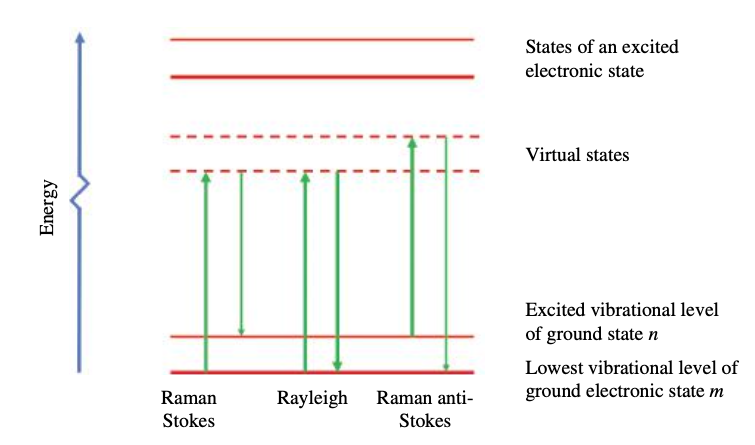
\includegraphics[width=1\linewidth]{Images/raman_energy_levels.png}
    \caption{The energy levels involved in Raman Stokes and Raman Anti-Stokes processes, from \cite{smith_modern_2019}.}
    \label{fig:raman_energy_levels}
\end{figure}

The Raman spectroscopy data for this project has been collected using a patented broadband coherent Raman spectroscopy device, which utilises stimulated Raman spectroscopy (SRS) to pump photons from the excited vibrational level to the ground state, increasing photon emission rates by up to a factor of $10^6$, enabling much faster data acquisition at microscopic resolutions \cite{prince_stimulated_2017}. By using picosecond laser pulses which disperse to have a wide frequency spectrum, it is also possible to conduct these measurements across multiple frequencies simultaneously, further increasing acquisition speed. A basic overview of the CRI system is shown in Figure \ref{fig:CRI_raman}.

\begin{figure}
    \centering
    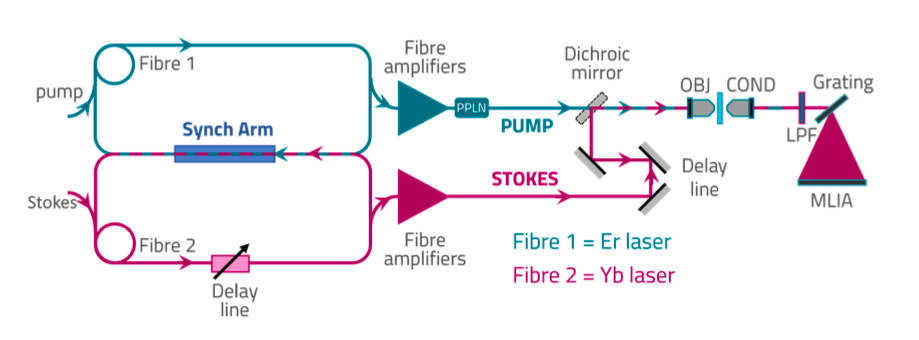
\includegraphics[width=1\linewidth]{Images/cri_raman.png}
    \caption{A schematic overview of the CRI SRS implementation. From CRI.}
    \label{fig:CRI_raman}
\end{figure}

\subsubsection{Second Harmonic Generation and Two-Photon Excitation Microscopies}
The polarisation of a material interacting with light is given by equation (\ref{eq:polarisation}) where $\chi^{(n)}$ is the $n$th order non-linear susceptibility tensor and $\mathbf E$ is the electric field vector \cite{shen_principles_2003}. The second term in equation (\ref{eq:polarisation}) corresponds to second harmonic generation (SHG), whereas the third term corresponds to two- and three-photon absorption and SRS processes.\\

\begin{equation} \label{eq:polarisation}
\mathbf{P}(\mathbf{k}, \omega) = \mathbf{P}^{(1)}(\mathbf{k}, \omega) + \mathbf{P}^{(2)}(\mathbf{k}, \omega) + \mathbf{P}^{(3)}(\mathbf{k}, \omega) + \dots
\end{equation}
With
\begin{align*}
\mathbf{P}^{(1)}(\mathbf{k}, \omega) &= \chi^{(1)}(\mathbf{k}, \omega) \cdot \mathbf{E}(\mathbf{k}, \omega), \\
\mathbf{P}^{(2)}(\mathbf{k}, \omega) &= \chi^{(2)}(\mathbf{k} = \mathbf{k}_i + \mathbf{k}_j, \, \omega = \omega_i + \omega_j) \\
&\quad : \mathbf{E}(\mathbf{k}_i, \omega_i)\mathbf{E}(\mathbf{k}_j, \omega_j), \\
\mathbf{P}^{(3)}(\mathbf{k}, \omega) &= \chi^{(3)}(\mathbf{k} = \mathbf{k}_i + \mathbf{k}_j + \mathbf{k}_l, \, \omega = \omega_i + \omega_j + \omega_l) \\
&\quad : \mathbf{E}(\mathbf{k}_i, \omega_i)\mathbf{E}(\mathbf{k}_j, \omega_j)\mathbf{E}(\mathbf{k}_l, \omega_l).
\end{align*}

When incident on a highly polarisable and non-centrosymmetric molecule, two photons can combine upon scattering, causing SHG emission with double the frequency of the incident radiation \cite{perry_two-photon_2012}. Notably, the requirement for non-centrosymmetric environments is a consequence of the second-order symmetry of SHG term in equation (2). As a consequence, incidence on centrosymmetric molecules causes the signal to vanish \cite{chen_second_2012}. This makes SHG especially sensitive to fibrillar collagen in a range of tissues, with changes due to cancerous growths often detectable.\\

The use of two incident photon frequencies from the pump and Stokes beams combined with femptosecond laser pulses for SRS also enable two-photon excitation microscopy to be conducted, where both incident photons simultaneously induce excitations within the incident molecule, which can then be detected \cite{denk_two-photon_1990}. This method is important for cancer detection, as it provides increased imaging depth, can elucidate metabolism within living cells, and can also be conducted using lower energy photons, reducing the risk of photo-damage to a sample \cite{perry_two-photon_2012}. A summary of the energy processes within TPEF and SGH emissions are summarised in Figure \ref{fig:tpef_shg_energies}.
\begin{figure}
    \centering
    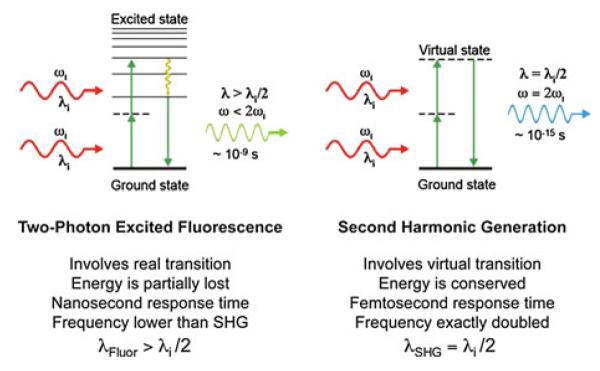
\includegraphics[width=1\linewidth]{Images/nihms-365614-f0001.jpg}
    \caption{A comparison of the energy processes in TPEF and SHG \cite{perry_two-photon_2012}.}
    \label{fig:tpef_shg_energies}
\end{figure}

\subsubsection{Fourier Transform Infrared (FTIR) Spectroscopy}
Infrared spectroscopy works by directing a broadband spectrum with wavenumbers ranging from around $400-4000 \text{ cm}^{-1}$  (for mid-IR spectroscopy) \cite{su_fourier_2020} onto a sample. This coherent spectrum then excites resonant vibrational modes within molecular bonds inside the sample, causing absorption of specific frequencies depending on the composition of the incident sample. This decreases the intensity relative to the baseline in the absorbed frequencies, therefore allowing a characteristic spectrum for each bond to be established. Modern devices use a Fourier transform-based (FTIR) interferogram approach \cite{griffiths_fourier_1983}, enabling high signal-to-noise (SNR) ratios to be achieved.\\

FTIR can detect biochemical compositions including nucleic acids, proteins, lipids and carbohydrates within biological samples by matching the observed spectra with known forms for different bonding types, functional groups and intermolecular interactions \cite{su_fourier_2020}. Typical absorption groups within biological samples are detailed in Table \ref{table:functional_groups}.

% Requires: \usepackage{array}
\begin{table}[h]
    \centering
    \begin{tabular}{|>{\centering}m{3.3cm}|>{\centering\arraybackslash}m{4cm}|}
    \hline
    \textbf{Wavenumber (cm\textsuperscript{-1})} & \textbf{Assignment} \\ 
    \hline
    3080--2800 & Anti-symmetric and symmetric C--H stretches from proteins and lipids \\ 
    \hline
    1745--1725 & Ester carbonyl of lipids \\ 
    \hline
    1700--1500 & Amide I and II groups in peptide linkages of proteins \\ 
    \hline
    1270--1080 & Anti-symmetric and symmetric C--O and P--O areas in DNA, RNA and phospholipids \\ 
    \hline
    1200--900 & Carbohydrate vibrations of glucose, fructose and glycogen \\ 
    \hline
    \end{tabular}
    \caption{\centering Assignments of Various Functional Groups Based on Wavenumber}
    \label{table:functional_groups}
\end{table}

\begin{figure*}[h]
    \centering
    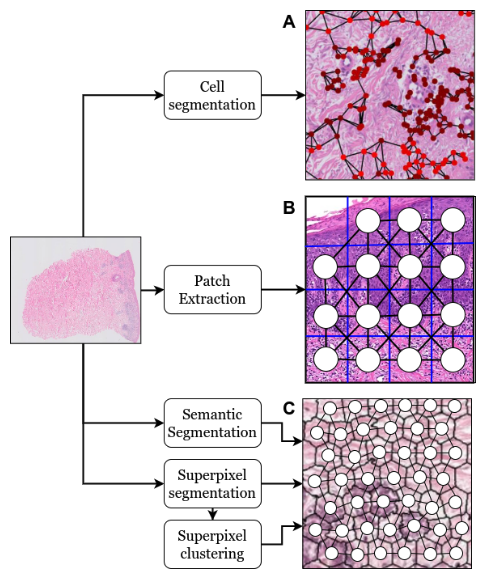
\includegraphics[width=0.5\linewidth]{Images/gnn_features.png}
    \caption{\centering Commonly used graph types in histopathology A) showing a cell graph, B) a patch graph and C) a tissue graph. From \cite{brussee_graph_2024}.}
    \label{fig:GNN_features}
\end{figure*}

\begin{figure*}[h]
    \centering
    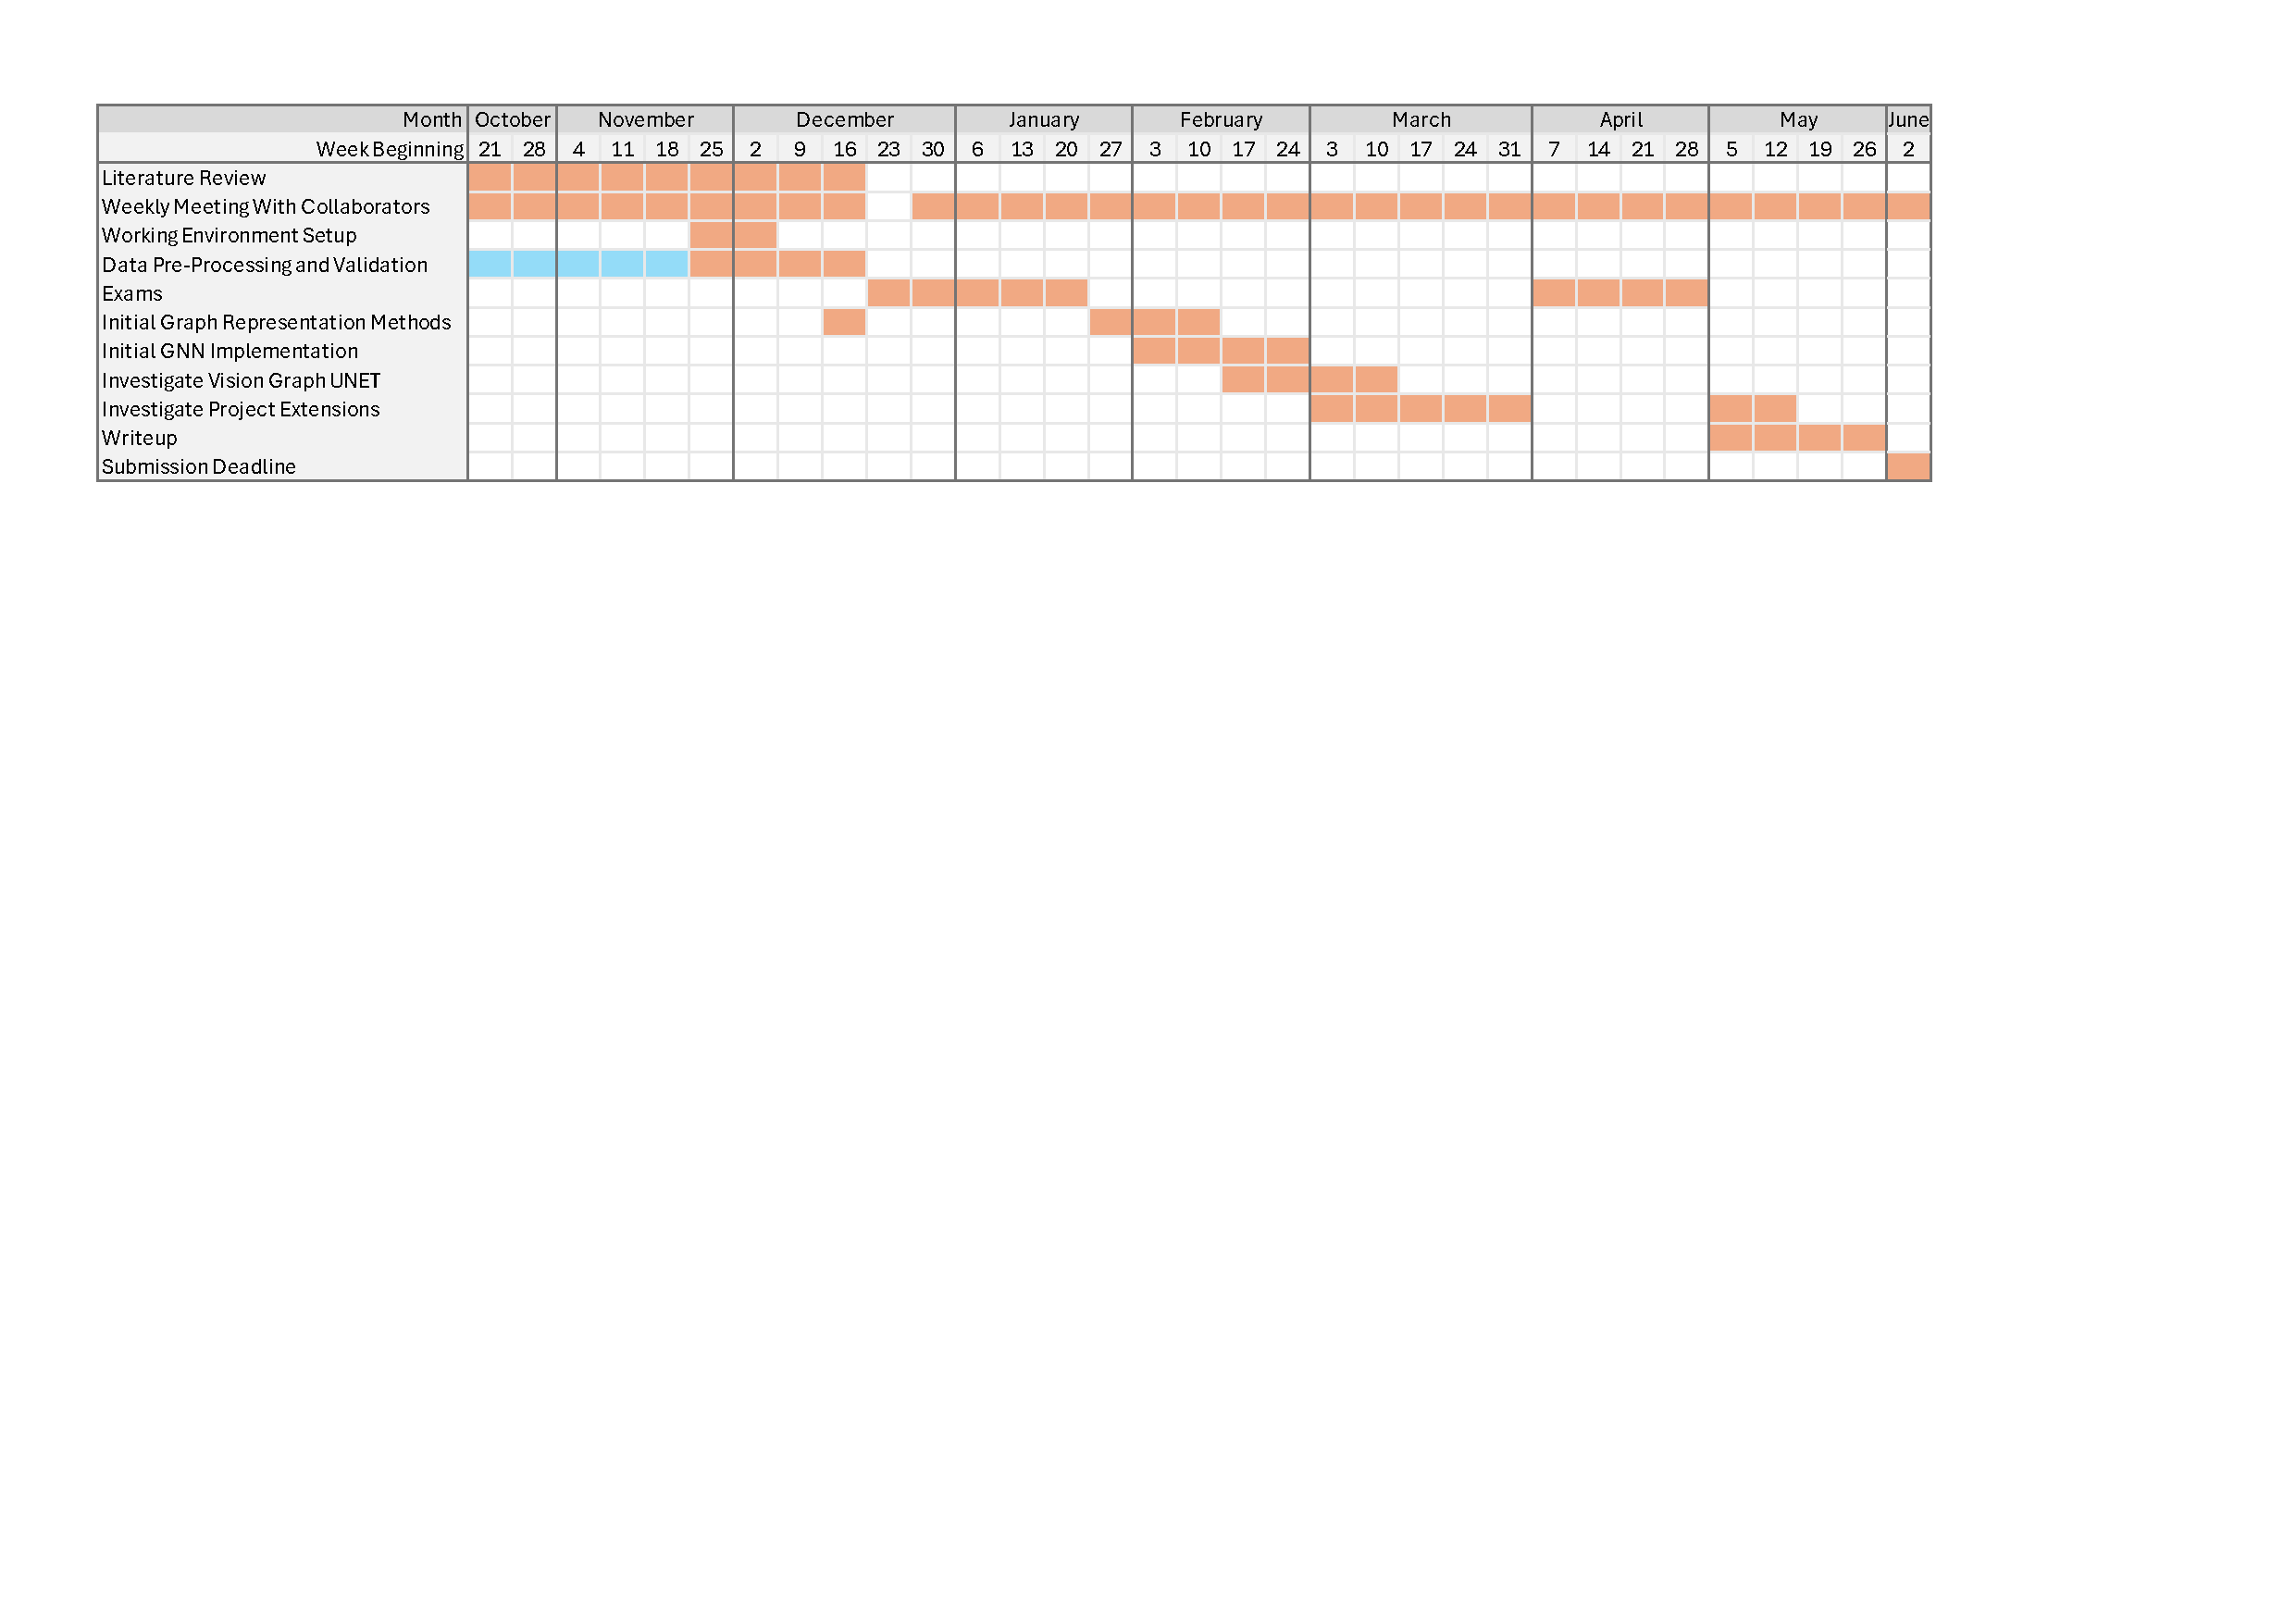
\includegraphics[width=1\linewidth]{Images/Part3ProjectPlanPDF.pdf}
    \caption{\centering Project timeline. Blue highlighting represents preparatory work done by members of the CHARM collaboration.}
    \label{fig:plan}
\end{figure*}

\subsection{Graph Neural Networks}
Here, we define a graph like in \cite{broadwater_graph_2025} as “data structures with elements expressed as nodes or vertices, and relationships between those elements, expressed as edges”. The intrinsic links within a graph are excellent for exploiting relationships between data. Traditionally, they are used in the context of systems with intrinsic connections, such as; the relationships between people on social media, where individuals can be encoded as vertices and the relationships between them encoded by edges; or maps, where street intersections can be stored as vertices and the kind of connections between each intersection (what type of road, speed limit etc.) can be encoded by the edges. By encoding a graph with a list of connected vertices and the weights of each connection, it is immediately seen that the ordering of such a list has no impact. Graph neural networks leverage this permutation invariance to encode and exchange information across a graph structure during the learning process \cite{broadwater_graph_2025}. \\




By including relational information within a graph, models can develop physical intuition \cite{sanchez-gonzalez_graph_2018, sanchez-gonzalez_learning_2020} and harness the topological structures in Biological imaging. It is thought that this approach can offer advantages over vision transformer models by learning context-aware representations between biologically relevant areas of spectra rather than arbitrary patches of these spectra \cite{brussee_graph_2024}. Furthermore, due to the large dataset sizes involved in histopathological imaging, images are usually split into patches for transformer model applications, producing bias. By modelling the whole image as a graph, memory requirements can be significantly reduced, allowing a GNN model to learn using the global structure of an image. Utilising the whole image representation in conjunction with graphs encoding smaller-scale features then allows for hierarchical modelling of each sample \cite{brussee_graph_2024}. Due to the entity-attachment qualities graphs encode, GNNs can also provide advantages in terms of explainability, although this work will not explore explainability in detail.\\


The data for this project shows distinctive characteristics, such as cell nuclei, so it is thought that by extracting relevant information from each spectra and encoding that information within a graph with sensible relational information, it should be possible to predict which regions are cancerous and which are not. The task of feature extraction, however, is sensitive, as we wish to encode all relevant information from the spectra within the graph. Therefore, multiple methods for feature extraction will be explored, beginning with basic segmentation approaches, tissue graphs and superpixels, as outlined in \cite{brussee_graph_2024} and depicted in Figure \ref{fig:GNN_features}. To extract the features for each vertex in these graphs, morphological features, CNNs or Vision transformers can be used. There has also been progress recently in using self-supervised learning for such representations, and this could also be investigated \cite{tendle_study_2021}. One particularly interesting method which automates this feature extraction to utilise GNNs is vision graph U-NETs \cite{jiang_vision_2024}, which this work will try to explore.

\begin{figure}[h]
    \centering
    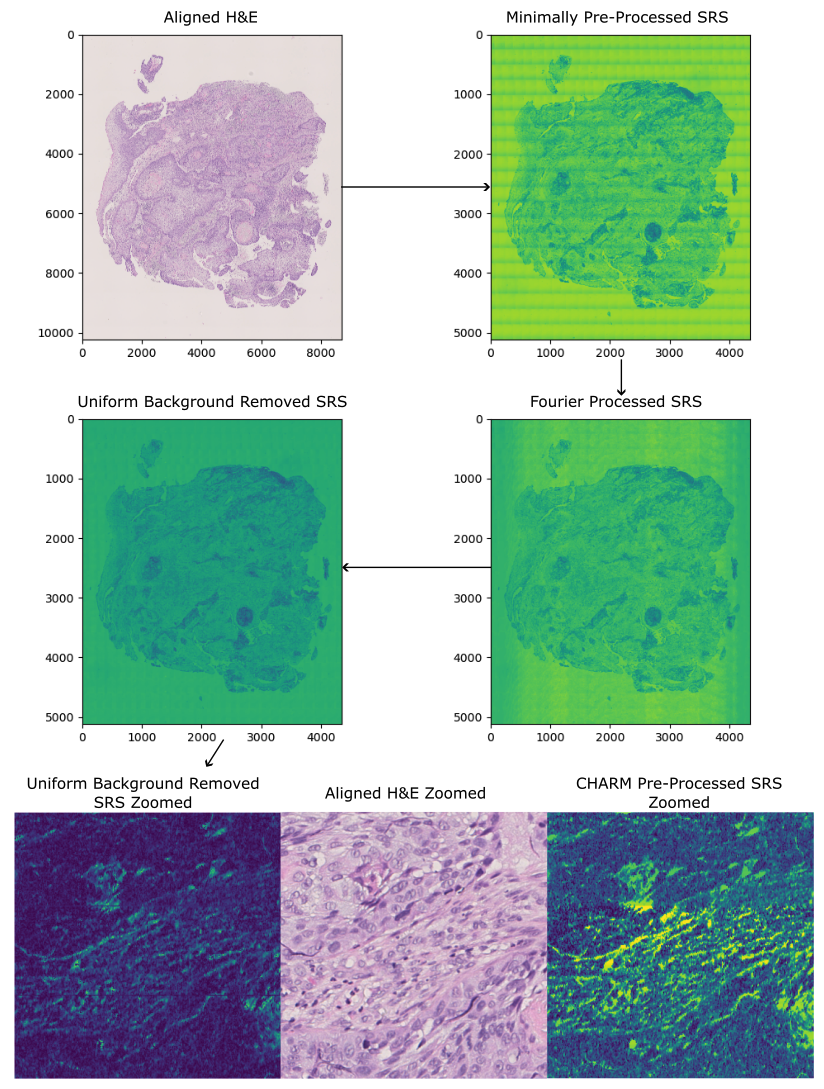
\includegraphics[width=1\linewidth]{Images/different_processing_compare.png}
    \caption{\centering Plots showing a comparison between the Fourier domain noise removal strategy and that used by the CHARM group. The HE images for the respective regions are also provided. Note that the large differences between the SRS signal and the HE image are expected, as we are only showing one of the 31 recorded SRS spectra for the sample.}
    \label{fig:different_process}
\end{figure}

\section{Project Status}
\subsection{Plan} \label{sec:plan}
The primary goal of this project is to assess the feasibility of applying GNNs to the CHARM and TROPHY datasets for automated cancer annotation. The steps towards this outcome are outlined in Figure \ref{fig:plan}. It is hoped that this method can be combined with the UNETR and UNET methods developed by projects in the previous academic year to achieve even stronger performance.

\subsection{Progress}
Initial progress with the project has been steady, with a good review of the literature undertaken. It is hoped that by the fourth week of December, all necessary literature to begin on GNN implementation will have been examined. Furthermore, access has been granted to the Kiiara machine owned by the Computational Biology group. This machine contains four Titan XP graphics cards, which should be sufficient for initial implementation and experimentation, but could be limiting when attempting training using the full datasets.\\

Good progress has also been made in data pre-processing, with members of the CHARM collaboration delivering aligned HE images and pre-processed SRS signals around mid-November. Notably, they used a different pre-processing method for the SRS signal than that detailed in the reports from last year \cite{vali_deep_2024, petrov_diagnosing_2024}. It has been noticed in data pre-processing for this work that implementing and expanding on the Fourier domain methods used last year gives similar, but notably different results - see Figure \ref{fig:different_process}. This is therefore an area which warrants further consideration. Potential avenues to explore include using the logarithm of intensity data, as they often cover many orders of magnitude, and taking ratios of SRS channel intensities in an attempt to remove focus-induced systematic errors.\\
 

There have, however, been some delays in data acquisition for the project. Although CHARM has provided SRS, TPEF, SHG and HE images, they have yet to begin the annotation process. This is due to a range of logistical issues, but they hope annotations can be completed in January. That should give plenty of time for this project. Furthermore, a subset of the TROPHY data seems to contain large processing artifacts not present in the original data. A revised version of this data has been requested, but there should be enough correct data to begin with.

\subsection{Extensions} \label{sec:extensions}
There are many exciting possibilities for extending this project, many of which have been mentioned in the above text, such as self-supervised learning for feature extraction during graph creation. The CHARM project is also trying to generate virtual HE images using the SRS, TPEF and SHG data, so it would be possible to explore whether GNNs can contribute positively to this task.

%most progress stuff here, but also mention delays in histrographic annotation and corrected TROPHY data acquisition
\section{Conclusion}
This project is an exciting fusion of state-of-the-art microscopy technology and machine learning applications to help improve the reliability and efficiency of cancer detection. Good progress has been made throughout Michaelmas term towards the objectives set out in the project timeline, and the project seems set on a good trajectory to begin GNN experimentation in the new year.